\chapter{Catene di Markov}

\section{Motivazioni}

Noi siamo partiti analizzando lo schema di Bernoulli e le Random Walk. In
entrambi la struttura del processo è determinata da:
\begin{enumerate}[label = \arabic*.]
    \item Somme: \(S_{n} = \sum_{i=1}^{n} X_{i} \) 
    \item \(X_{i}\) sono i.i.d.
    \item Regolarità / Integrabilità delle \(X_{i}\) 
\end{enumerate}
E domande sensate potrebbero essere cosa succede indebolendo una o più dei
precedenti punti.

Nella generalizzazione proposta da Markov, il fulcro è l'indebolimento della
nozione di \textbf{indipendenza}.

\section{Catena di Markov}

Il setting è: una famiglia \(\{X_{n}\}_{n \in \mathbb{N}} \) di variabili
aleatorie e uno spazi odiscreto \(E\) detto \emph{spazio degli stati}. 

\begin{definition}{Proprietà di Markov}
    Nel setting precedentemente presentato, vale la proprietà di Markov se
    \(\forall \{X_{0}, X_{1}, \dots, X_{n}, y\} \in E\) vale che
    \begin{equation}\label{eq:propr_markov}
       \mathbb{P}{(X_{n+1}
      = y \;|\; X_{0} = n_{0}, \dots, X_{n} = x_{n})} = \mathbb{P}{(X_{n+1} = y
  \;|\; X_{n} = x_{n})}
    \end{equation}

Se vale~\eqref{eq:propr_markov} allora la catena si dice di Markov. Inoltre la
catena è detta \emph{omogenea} se
\[
  \mathbb{P}{(X_{n+1} = y \;|\; X_{n} = x_{n})} = \mathbb{P}{(X_{1} = y \;|\;
  X_{0} = x_{n})}
\]

\end{definition}

\begin{example}{}
    \(S_{n}\) per lo schema di Bernoulli è una catena di Markov. (\(X_{n}\) con
    la distribuzione più semplice)
\end{example}

\begin{example}{}
    \(E = \{0, 1\} \) è la scelta con \(E\) più semplice. Devo dunque assegnare
    4 probabilità:
    \begin{align*}
    &\mathbb{P}{(X_{1} = 0 \;|\; X_{0} = 0)} = 1-p
    &\mathbb{P}{(X_{1} = 1 \;|\; X_{0} = 0)} = p\\
    &\mathbb{P}{(X_{1} = 0 \;|\; X_{0} = 1)} = q
    &\mathbb{P}{(X_{1} = 1 \;|\; X_{0} = 1)} = 1-q
    \end{align*}

\begin{center}
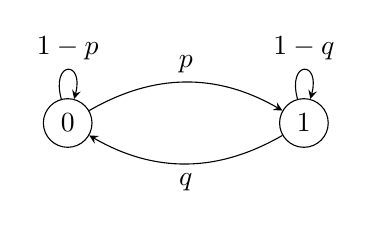
\begin{tikzpicture}[>=stealth, node distance=3cm]

    % Nodes
    \node[circle, draw] (A) {0};
    \node[circle, draw, right of=A] (B) {1};

    % Arrows between states
    \draw[->] (A) to[bend left] node[above] {$p$} (B);
    \draw[->] (B) to[bend left] node[below] {$q$} (A);

    % Self-loops
    \draw[->] (A) to[loop above] node {$1-p$} (A);
    \draw[->] (B) to[loop above] node {$1-q$} (B);

\end{tikzpicture}
\end{center}

    Dunque per descrivere la catena basta presentare i 4 oggetti
    \[
      P = \begin{pmatrix}
          P{(0,0)} & P{(0,1)} \\
          P{(1,0)} & P{(1,1)}
      \end{pmatrix} = \begin{pmatrix}
          1-p & p \\
          q & 1-q
      \end{pmatrix}
    \]
    che è una matrice \(\{P{(x,y)}\}_{E \times  E}  \) con somme sulle righe 1.
    Queste matrici si dicono \textbf{stocastiche}.
\end{example}

Più in generale rispetto all'esempio precedente, abbiamo che
\begin{definition}{Matrice stocastica}
   Una matrice stocastica è una matrice \(\{P{(x, y)}\} _{E \times  E} \), ossia
   \(P : E \times E \to [0, 1]\) è data da 
   \[
     P{(x, y)} = \mathbb{P}{(X_{1} = x \;|\; X_{0} = y)}
   \]
   che è chiaramente tale che ha somma sulle righe 1.
   
   Questa è dette \textbf{matrice di transizione}
\end{definition}

è equivalente dare la matrice di transizione o il grafo di adiacenza, dove
normalmente vengono omessi gli archi allo stesso vertice (loop).

\begin{example}[Schema di Bernoulli]
    \(E = \mathbb{N}\) e \(\{S_{n}\}_{n \in \mathbb{N}} \) sono le v.a. La
    ``matrice'' di transizione è
    \[
      \begin{pmatrix}
          1-p & p & 0 & 0 & \dots \\
          0 & 1-p & p & 0 & \dots \\
          0 & 0 & 1-p & p & \dots \\
          \vdots & \vdots & \vdots & \vdots & \ddots
      \end{pmatrix}
    \]
\end{example}

\begin{eser}{Random Walk}
    Disegna il grafo di adiacenza e presenta la matrice di transizione della
    passeggiata aleatoria
\end{eser}

\begin{proposition}{}
    Date \(\{\xi_{n} \} _{n \in \mathbb{N}} \) v.a. i.i.d. su \(F\). Sia \(f : E
    \times F \to E\) misurabile e \(X_{0} : \Omega \to E\) indipendente dalle
    \(\xi_n\). Allora la famiglia \(\{X_{n}\} _{n \in \mathbb{N}} \) definite da 
    \[
        X_{n+1} = f{(X_{n}, \xi_{n+1} )} \quad n \ge  0
    \]
    è una Catena di Markov.
\end{proposition}

\begin{remark}{}
    In questa scrittura la famiglia \(\{X_{n}\} \) non ha nessun tipo di
    struttura (tipo somma).
\end{remark}

\begin{proof}{}
    Dimostriamo la proprietà di Markov.
    \begin{align*}
        &\mathbb{P}{(X_{n+1}) = y \;|\; X_{0} = x_{0}, \dots, X_{n} = x_{n}} =
        \\
        = &\mathbb{P}{(f{(X_{n}, \xi_{n+1} )} = y \;|\; X_{0} = x_{0}, \dots,
        X_{n} = x_{n})}
    \end{align*} 

    Osservo che l'evento \(\{X_{0} = x_{0}, \dots, X_{n} = x_{n}\} \) dipende
    solo da \(X_{0}\), \(\xi_{1}, \dots, \xi_n\) e \textbf{non} dipende da
    \(\xi_{n+1} \). Segue che \(\{f{(x_{n}, \xi_{n+1} )} = y\} \coprod \{X_{0} =
    x_{0}, \dots, X_n = x_{n}\} \) quindi 
    \[
      \mathbb{P}{(X_{n+1}  = y \;|\; X_{0} = x_{0}, \dots, X_{n} = x_{n})} =
      \mathbb{P}{(f{(x_{n}, \xi_{n+1} )} = y)}
    \]
    D'altra parte:
    \[
      \mathbb{P}{(f{(X_{n}, \xi_{n+1} )} = y \;|\; X_{n} = x_{n})} =
      \mathbb{P}{(f{(x_{n}, \xi_{n+1} )} = y)}
    \]
\end{proof}
\begin{remark}{}
    \(\mathbb{P}{(f{(x_{n}, \xi_{n+1} )} = y)}\) non dipende da \(n\), dunque
    questa catena di Markov è omogenea, dunque posso definire la matrice di
    transizione:
    \[
      P{(x, y)} = \mathbb{P}{(f{(x, \xi_{1})} = y)}
    \]
\end{remark}
\begin{remark}{}
    Il dato di uno spazio \(E\), una funzione \(f\) (deterministica) e una
    successione \(\xi_n\), e eventualmente un dato iniziale \(X_{0}\),
    è chiamato \textbf{sistema dinamico aleatorio} (RDS).
\end{remark}

Si può dimostrare in realtà che per ogni catena di markov esiste un sistema
dinamico aleatorio che la definisce, anche se potrebbe non essere unico.





